\makeatletter
\pgfmathdeclarefunction{erf}{1}{%
    \begingroup
    \pgfmathparse{#1 > 0 ? 1 : -1}%
    \edef\sign{\pgfmathresult}%
    \pgfmathparse{abs(#1)}%
    \edef\x{\pgfmathresult}%
    \pgfmathparse{1/(1+0.3275911*\x)}%
    \edef\t{\pgfmathresult}%
    \pgfmathparse{%
        1 - (((((1.061405429*\t -1.453152027)*\t) + 1.421413741)*\t
        -0.284496736)*\t + 0.254829592)*\t*exp(-(\x*\x))}%
    \edef\y{\pgfmathresult}%
    \pgfmathparse{(\sign)*\y}%
    \pgfmath@smuggleone\pgfmathresult%
    \endgroup
}
%dep
%subfig
\begin{figure}[htp]
    \centering
    \captionsetup{format=hang} % hanging captions
    \subfloat[Threshold Step]{
        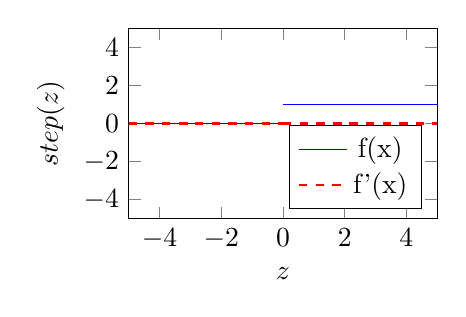
\begin{tikzpicture}
            \label{fig:threshold}
            \begin{axis}
                [width=5.5cm,height=4cm,ylabel=$step(z)$,xlabel=$z$,ymin=-5.0,ymax=5.0,xmin=-5,xmax=5,
                legend style={at={(0.95,0.05)},anchor=south east},]
                \addplot[blue,smooth, domain=-5:0] {0};
                \addplot[red,dashed, thick, domain=-5:0] {0};
                \addplot[blue,smooth, domain=-0:5] {1};
                \addplot[red,dashed, thick, domain=-0:5] {0};
                \addlegendentry{f(x)}
                \addlegendentry{f'(x)}
            \end{axis}
        \end{tikzpicture}
    }
    \subfloat[Linear]{
        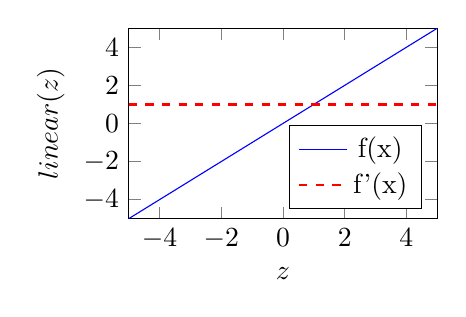
\begin{tikzpicture}
            \label{fig:linear}
            \begin{axis}
                [width=5.5cm,height=4cm,ylabel=$linear(z)$,xlabel=$z$,ymin=-5.0,ymax=5.0,xmin=-5,xmax=5,
                legend style={at={(0.95,0.05)},anchor=south east},]
                \addplot[blue,smooth] {x};
                \addlegendentry{f(x)}
                \addplot[red,dashed, thick] {1};
                \addlegendentry{f'(x)}
            \end{axis}
        \end{tikzpicture}
    }
    \subfloat[Sigmoid]{
        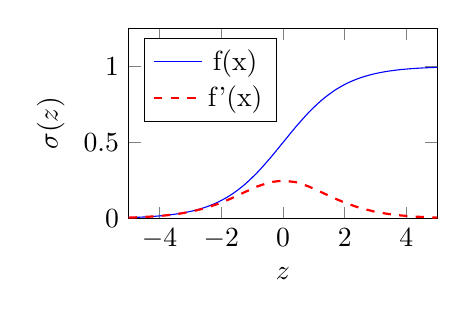
\begin{tikzpicture}
            \label{fig:sigmoid}
            \begin{axis}
                [width=5.5cm,height=4cm,ylabel=$\sigma(z)$,xlabel=$z$,ymin=0,ymax=1.25,xmin=-5,xmax=5,
                legend style={at={(0.05,0.95)},anchor=north west},]
                \addplot[blue,smooth] {1/(1+exp(-x))};
                \addlegendentry{f(x)}
                \addplot[red, dashed, thick] {1/(1+exp(-x)) * (1-1/(1+exp(-x)))};
                \addlegendentry{f'(x)}
            \end{axis}
        \end{tikzpicture}
    }\\
    \subfloat[Hyperbolic tangent]{
        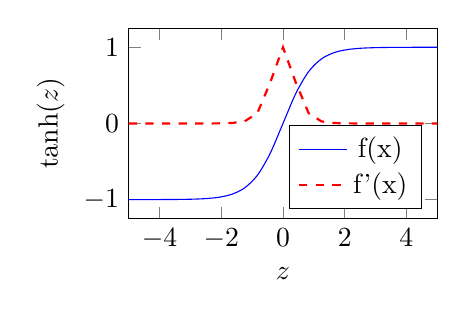
\begin{tikzpicture}
            \label{fig:hyperbolic_tangent}
            \begin{axis}
                [width=5.5cm,height=4cm,ylabel=$\tanh(z)$,xlabel=$z$,ymin=-1.25,ymax=1.25,xmin=-5,xmax=5, legend style={at={(0.95,0.05)},anchor=south east},]
                \addplot[blue,smooth] {tanh(x)};
                \addlegendentry{f(x)}
                \addplot[red,dashed, thick] {1/cosh(2*x)*1/cosh(2*x)};
                \addlegendentry{f'(x)}
            \end{axis}
        \end{tikzpicture}
    }
    \subfloat[ReLU]{
        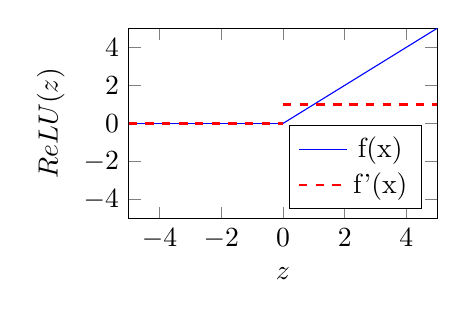
\begin{tikzpicture}
            \label{fig:relu}
            \begin{axis}
                [width=5.5cm,height=4cm,ylabel=$ReLU(z)$,xlabel=$z$,ymin=-5.0,ymax=5.0,xmin=-5,xmax=5,
                legend style={at={(0.95,0.05)},anchor=south east},]
                \addplot[blue,smooth, domain=-5:0] {0};
                \addplot[red,dashed, thick, domain=-5:0] {0};
                \addplot[blue,smooth, domain=-0:5] {x};
                \addplot[red,dashed, thick, domain=-0:5] {1};
                \addlegendentry{f(x)}
                \addlegendentry{f'(x)}
            \end{axis}
        \end{tikzpicture}
    }
    \subfloat[Leaky ReLU]{
        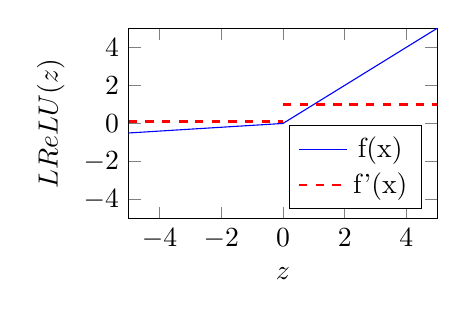
\begin{tikzpicture}
            \label{fig:lrelu}
            \begin{axis}
                [width=5.5cm,height=4cm,ylabel=$LReLU(z)$,xlabel=$z$,ymin=-5.0,ymax=5.0,xmin=-5,xmax=5,
                legend style={at={(0.95,0.05)},anchor=south east},]
                \addplot[blue,smooth, domain=-5:0] {0.1*x};
                \addplot[red,dashed, thick, domain=-5:0] {0.1};
                \addplot[blue,smooth, domain=-0:5] {x};
                \addplot[red,dashed, thick, domain=-0:5] {1};
                \addlegendentry{f(x)}
                \addlegendentry{f'(x)}
            \end{axis}
        \end{tikzpicture}
    }\\
    \subfloat[GELU]{
        \begin{tikzpicture}
            \label{fig:gelu}
            \begin{axis}
                [width=5.5cm,height=4cm,ylabel=$GELU(z)$,xlabel=$z$,ymin=-5.0,ymax=5.0,xmin=-5,xmax=5,
                legend style={at={(0.95,0.05)},anchor=south east},]
                \addplot[blue,smooth] {x * 0.5 * (1 + erf(x /sqrt(2)))};
                \addplot[red,dashed, thick] {0.5 * (1 + erf(x /sqrt(2))) + 1/sqrt(2*pi) * (exp(-x*x/2))};
                \addlegendentry{f(x)}
                \addlegendentry{f'(x)}
            \end{axis}
        \end{tikzpicture}
    }
    \subfloat[Swish]{
        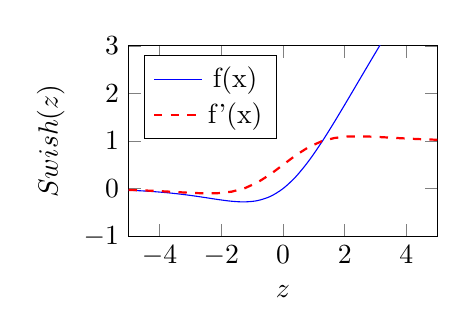
\begin{tikzpicture}
            \label{fig:swish}
            \begin{axis}
                [width=5.5cm,height=4cm,ylabel=$Swish(z)$,xlabel=$z$,ymin=-1,ymax=3.0,xmin=-5,xmax=5,
                legend style={at={(0.05,0.95)},anchor=north west},]
                \addplot[blue,smooth] {x*(1/(1+exp(-x)))}; % f (x) + σ (x) (1 − f (x))
                \addlegendentry{f(x)}
                \addplot[red, dashed, thick] {x/(1+exp(-x)) + 1/(1+exp(-x)) * (1-x/(1+exp(-x)))};
                \addlegendentry{f'(x)}
            \end{axis}
        \end{tikzpicture}
    }
    \subfloat[SIREN]{
        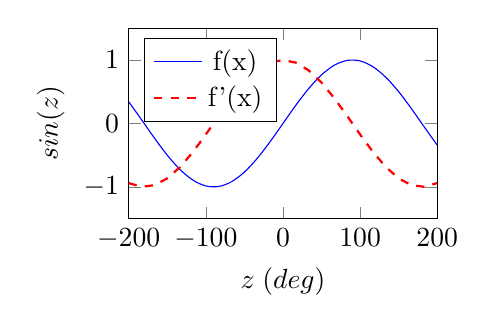
\begin{tikzpicture}
            \label{fig:siren}
            \begin{axis}
                [width=5.5cm,height=4cm,ylabel=$sin(z)$,xlabel=$z\;\text{(deg)}$,ymin=-1.5,ymax=1.5,xmin=-200,xmax=200,
                legend style={at={(0.05,0.95)},anchor=north west},]
                \addplot[blue,smooth,domain=-200:200] {sin(x)}; % f (x) + σ (x) (1 − f (x))
                \addlegendentry{f(x)}
                \addplot[red, dashed, thick,domain=-200:200] {cos(x)};
                \addlegendentry{f'(x)}
            \end{axis}
        \end{tikzpicture}
    }
    \caption[Activation functions.]{\textbf{Activation functions} used in \gls{DL}, included for results in their performance or historic significance in the applications of artificial neural networks.}
    \label{fig:activation-functions}
\end{figure}